\documentclass[aspectratio=1610]{beamer}
%\documentclass[aspectratio=1610, handout]{beamer}
\usepackage[utf8]{inputenc}
\usepackage{ragged2e}
\usepackage{xcolor}
\usepackage[italian]{babel}
\usepackage{multirow}
\usetheme[progressbar=frametitle,titleformat=smallcaps]{metropolis}
\setbeamertemplate{frame numbering}[fraction]
\setbeamercovered{dynamic}
\definecolor{rosso}{RGB}{255, 0, 0}
\definecolor{giallo}{RGB}{254,212,23}
\hypersetup{colorlinks=true,linkcolor=black,urlcolor=rosso}
\setbeamercolor{palette primary}{fg=black, bg=giallo}
\setbeamercolor{background canvas}{bg=white}
\setbeamercolor{normal text}{fg=black}
\setbeamercolor{progress bar}{fg=rosso}
\setbeamercolor{framesubtitle}{fg=rosso}
\setbeamercolor{normal text .dimmed}{fg=giallo}
\setbeamercolor{block title alerted}{fg=rosso, bg=giallo}
\setbeamerfont{caption}{size=\tiny}
\setbeamerfont{caption name}{size=\tiny}
\setlength{\abovecaptionskip}{0pt}
\makeatletter
\metroset{block=fill}
\setlength{\metropolis@progressinheadfoot@linewidth}{1pt} 
\setlength{\metropolis@progressonsectionpage@linewidth}{1pt}
\setlength{\metropolis@titleseparator@linewidth}{1pt}
\makeatother

\title{ARCHITETTURE E SERVIZI DI RETE}
\subtitle{Client-Server, evoluzione e servizi di Internet}
\date{}
\institute{\textit{
        Fonti:
        \begin{itemize}
            \item[-] \href{https://it.wikipedia.org/wiki/Server}{Wikipedia}
            \item[-] \href{https://www.fastweb.it/fastweb-plus/digital-dev-security/web-3-0-cos-e-cosa-sappiamo/}{Fastweb Plus}
        \end{itemize}
    }
}

\begin{document}

\begin{frame}[plain, noframenumbering]
    \titlepage
\end{frame}

\section{ARCHITETTURE DI RETE}

\begin{frame}{CLIENT - SERVER}
    \only<1 | handout:0>{\begin{figure}
        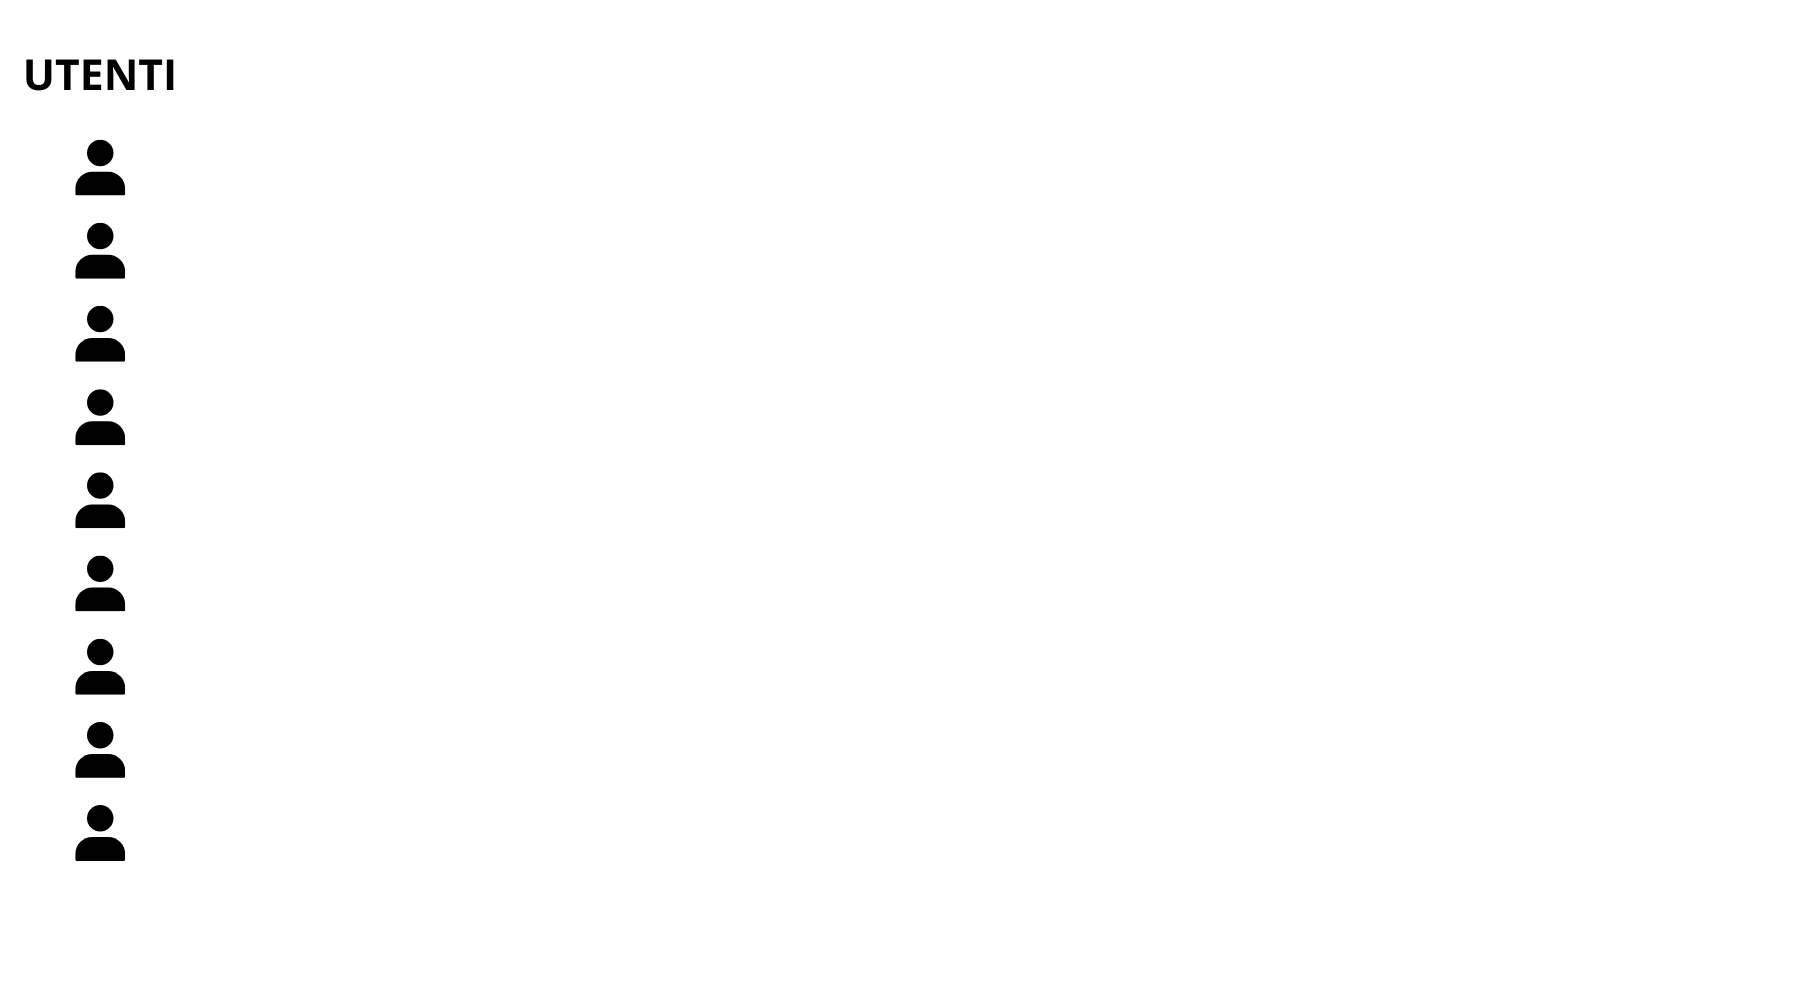
\includegraphics[width=\linewidth]{img/client-server1.png}
        \caption{{creata con \href{https://www.canva.com/}{Canva}}}
    \end{figure}}
    \only<2 | handout:0>{\begin{figure}
        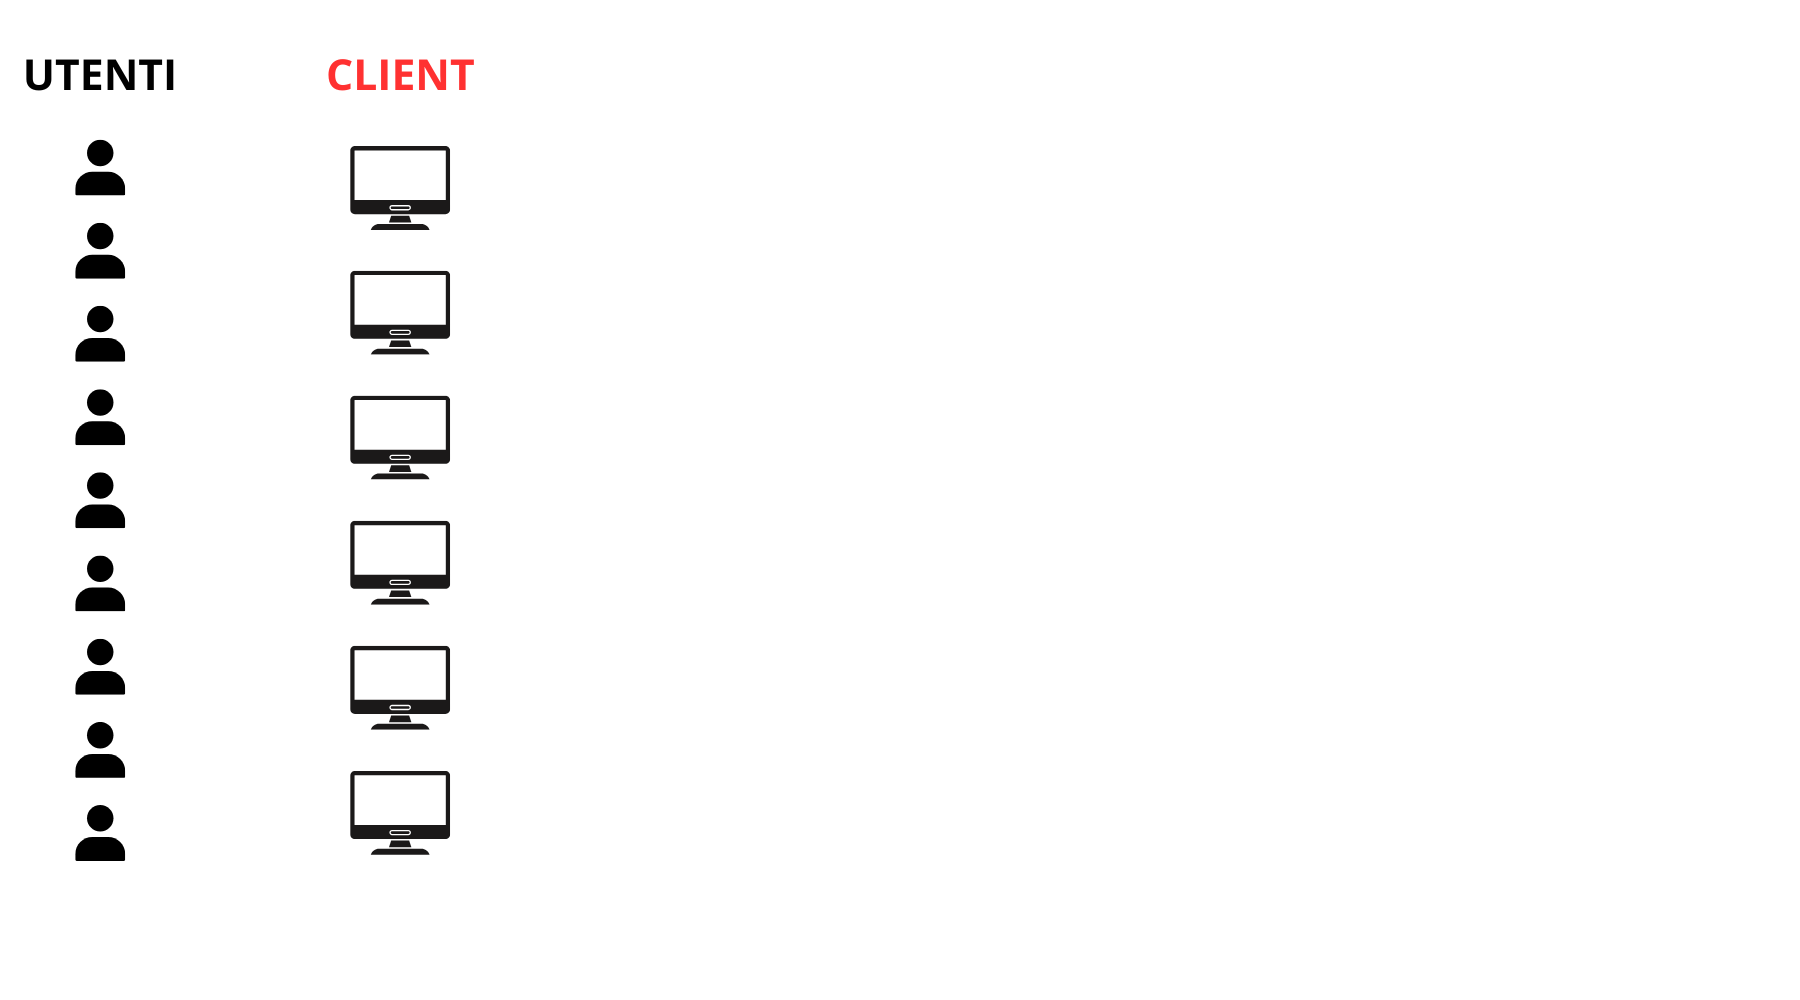
\includegraphics[width=\linewidth]{img/client-server2.png}
        \caption{{creata con \href{https://www.canva.com/}{Canva}}}
    \end{figure}}
    \only<3 | handout:0>{\begin{figure}
        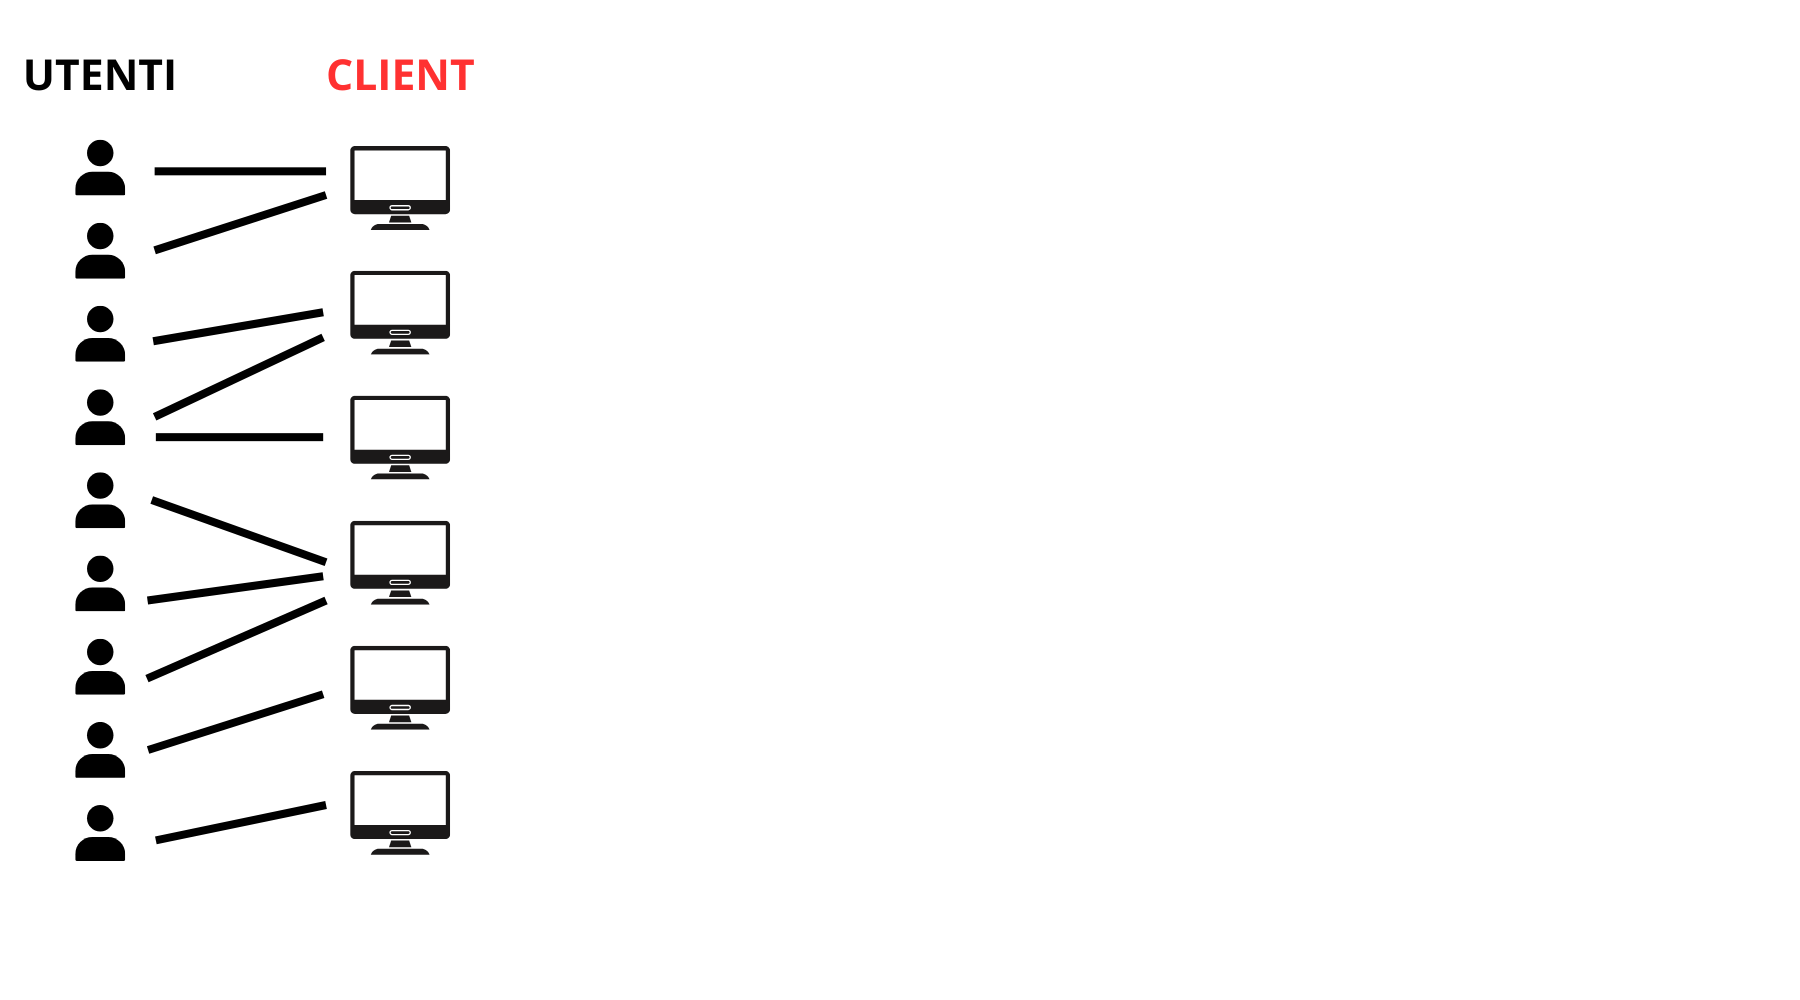
\includegraphics[width=\linewidth]{img/client-server3.png}
        \caption{{creata con \href{https://www.canva.com/}{Canva}}}
    \end{figure}}
    \only<4 | handout:0>{\begin{figure}
        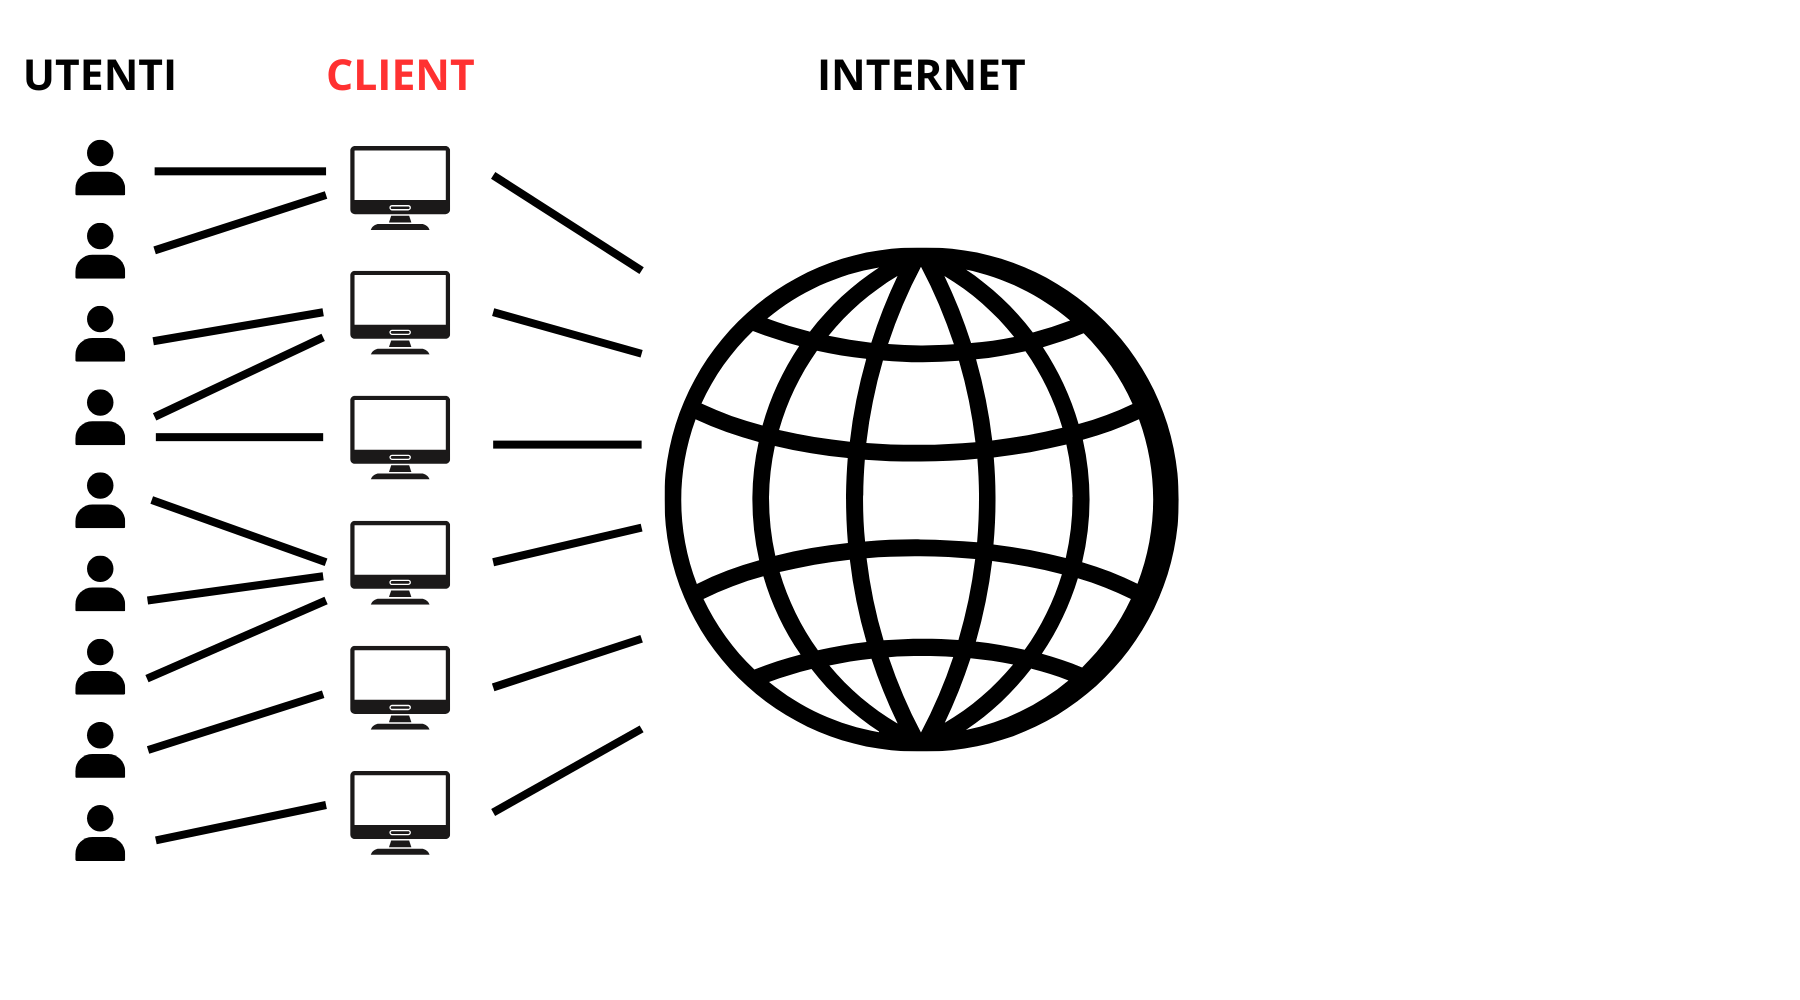
\includegraphics[width=\linewidth]{img/client-server4.png}
        \caption{{creata con \href{https://www.canva.com/}{Canva}}}
    \end{figure}}
    \only<5 | handout:1>{\begin{figure}
       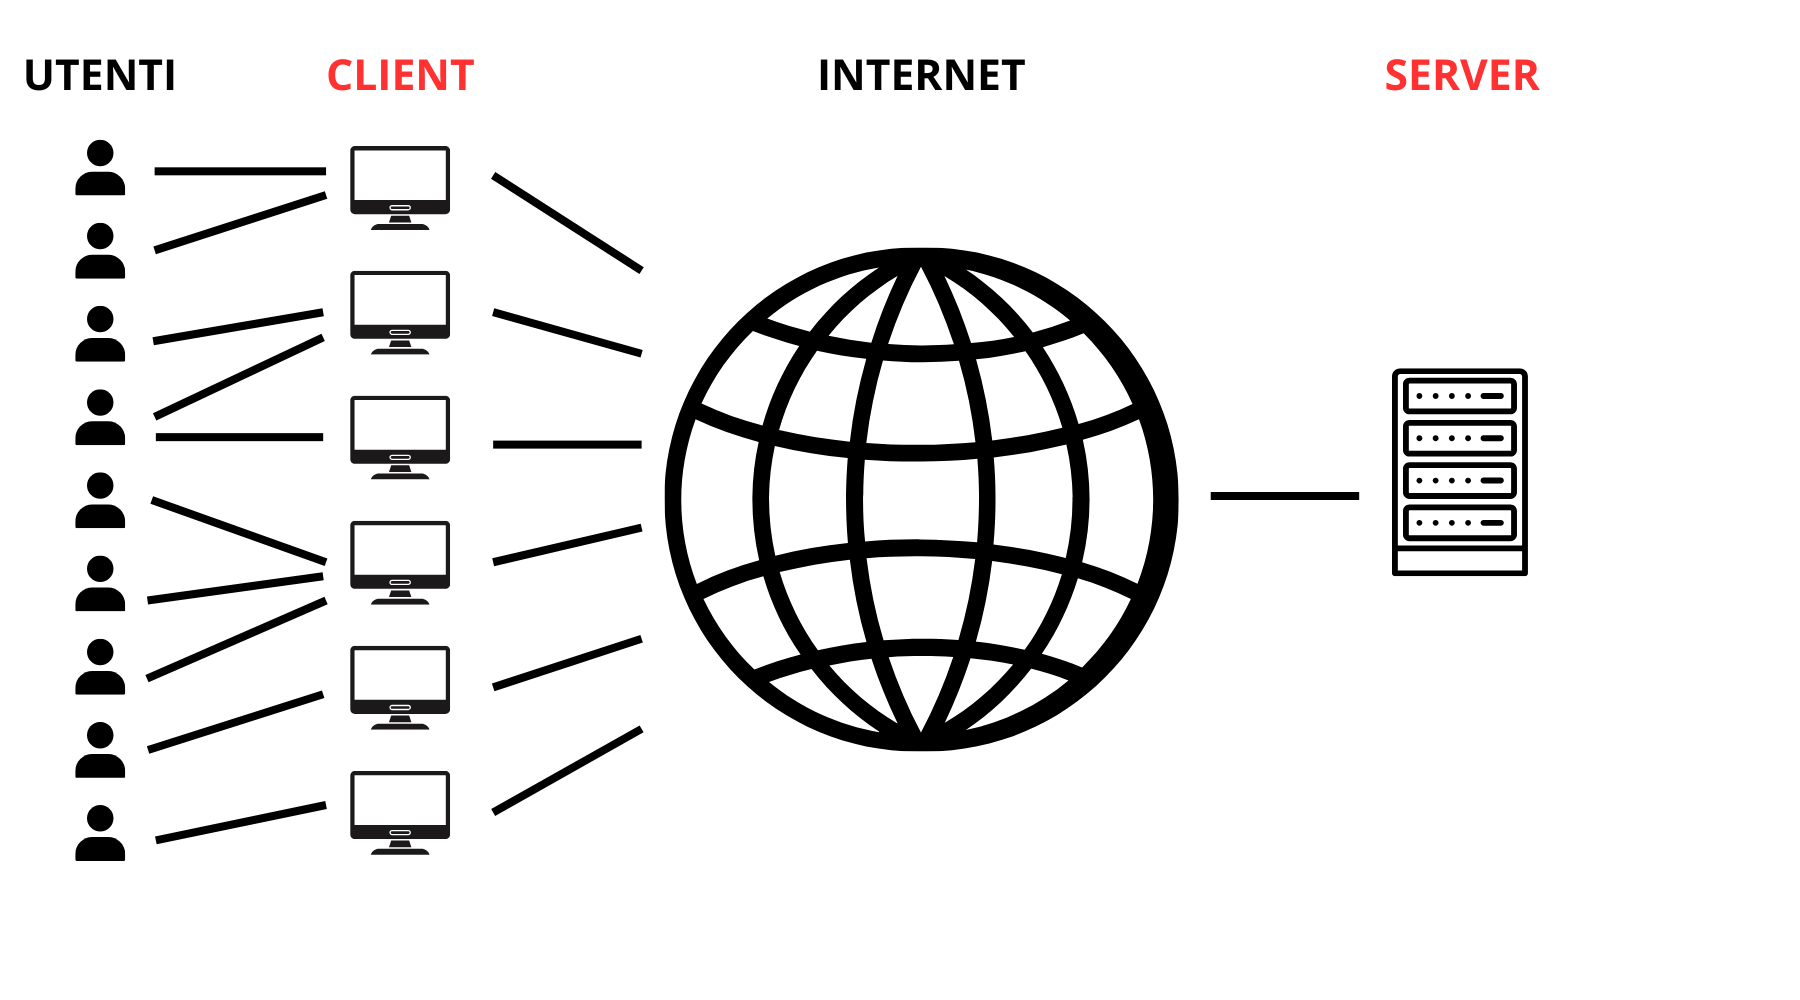
\includegraphics[width=\linewidth]{img/client-server5.png}
       \caption{{creata con \href{https://www.canva.com/}{Canva}}}
    \end{figure}}
    \only<6 | handout:2>{\begin{figure}
       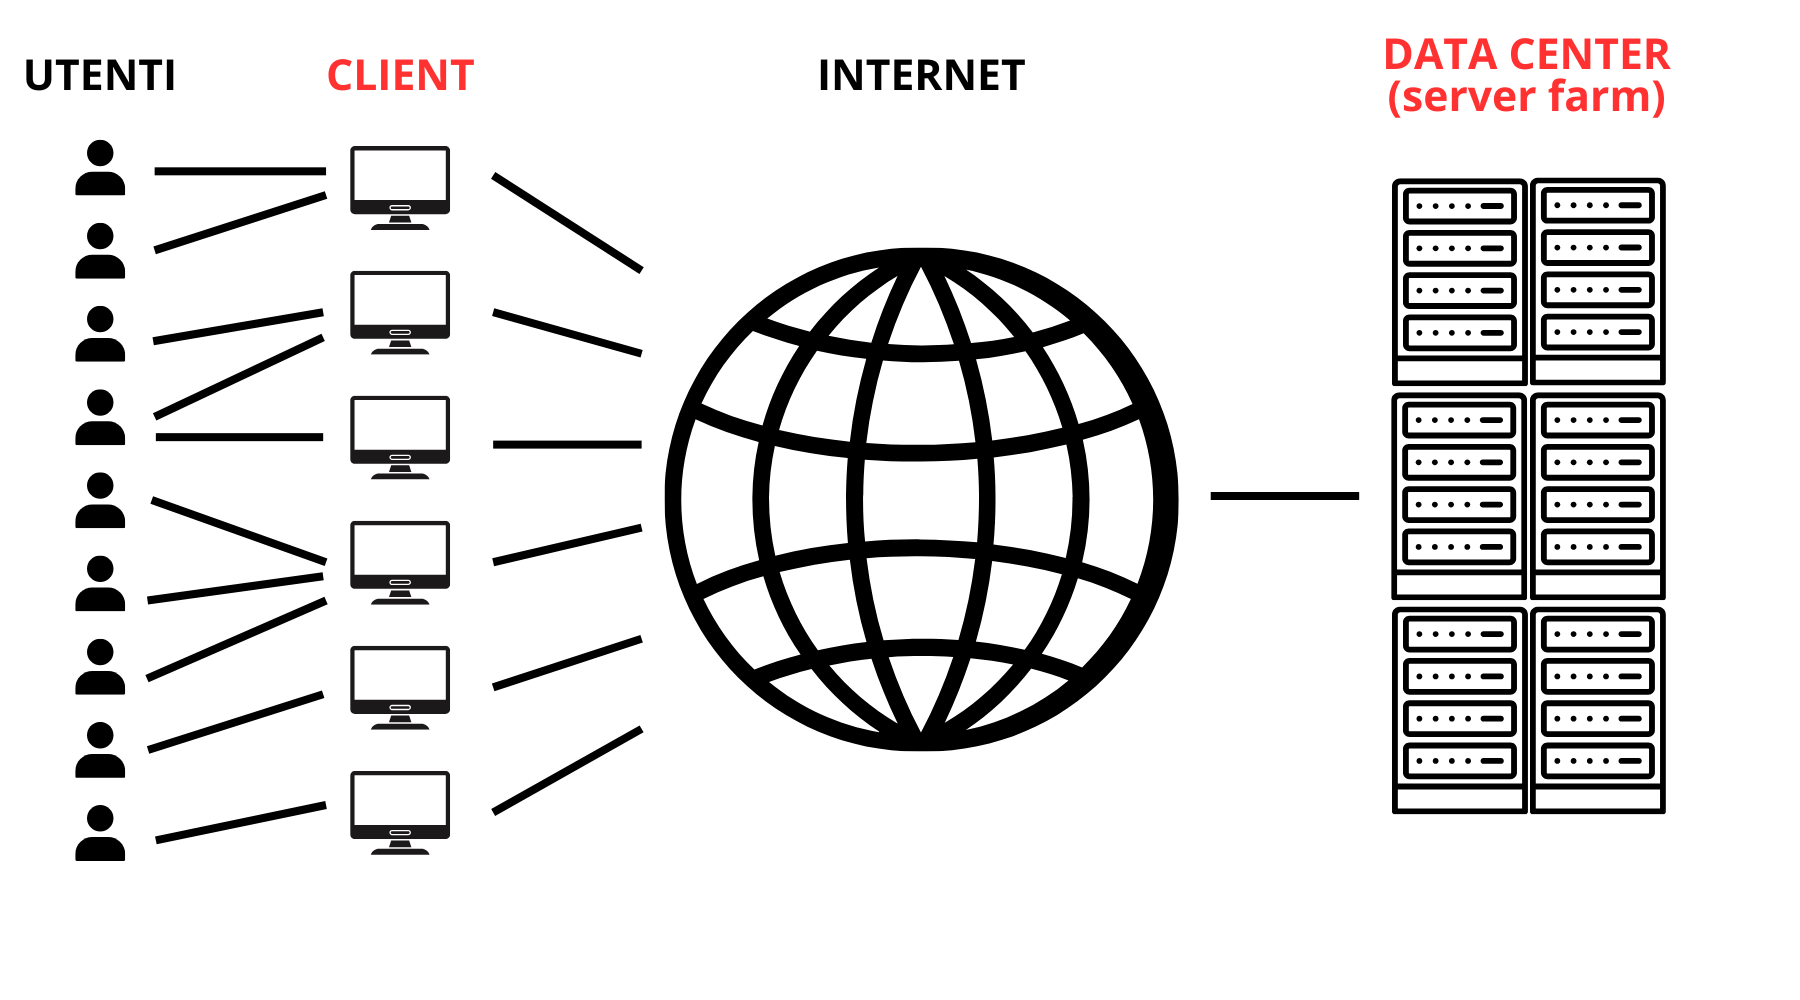
\includegraphics[width=\linewidth]{img/client-server6.png}
       \caption{{creata con \href{https://www.canva.com/}{Canva}}}
    \end{figure}}
\end{frame}

\begin{frame}{SERVER}
    \begin{columns}
        \column{.5\textwidth}
            \begin{alertblock}{DEFINIZIONE}
                \begin{minipage}{0.96\linewidth}
                    \justifying
                    Il termine \textbf{Server} indica un componente hardware che attraverso software specifico 
                    eroga servizi. I Server adottano accorgimenti volti a garantire alta affidabilità, 
                    continuità di servizio (disponibilità), robustezza ai guasti e alta sicurezza.
                    \begin{itemize}
                        \item Hardware con prestazioni elevate ed elementi ridondanti (dischi \href{https://it.wikipedia.org/wiki/RAID}{RAID});
                        \item Protezione fisica ("sala server");
                        \item Connessione di rete preferenziale ad alta prestazione;
                        \item Climatizzazione.
                    \end{itemize}
                    \tiny{\textbf{Curiosità}}\\
                    \tiny{\href{https://www.datacentermap.com/italy/}{Data Center in Italia}}
                \end{minipage}
            \end{alertblock}
        \column{.5\textwidth}
            \begin{itemize}
                \item \textbf{Server web}
                \item \textbf{Server di posta elettronica}
                \item \textbf{Server di messaggistica istantanea}
                \item \textbf{Server per i social network}
                \item \textbf{Server gaming}
                \item \textbf{Server cloud di memorizzazione}
                \item \textbf{Server cloud computing}
                \item \textbf{...}
            \end{itemize}
    \end{columns}
\end{frame}

\begin{frame}{PEER TO PEER (P2P)}
    \begin{columns}
        \column{.8\textwidth}
        \begin{figure}
            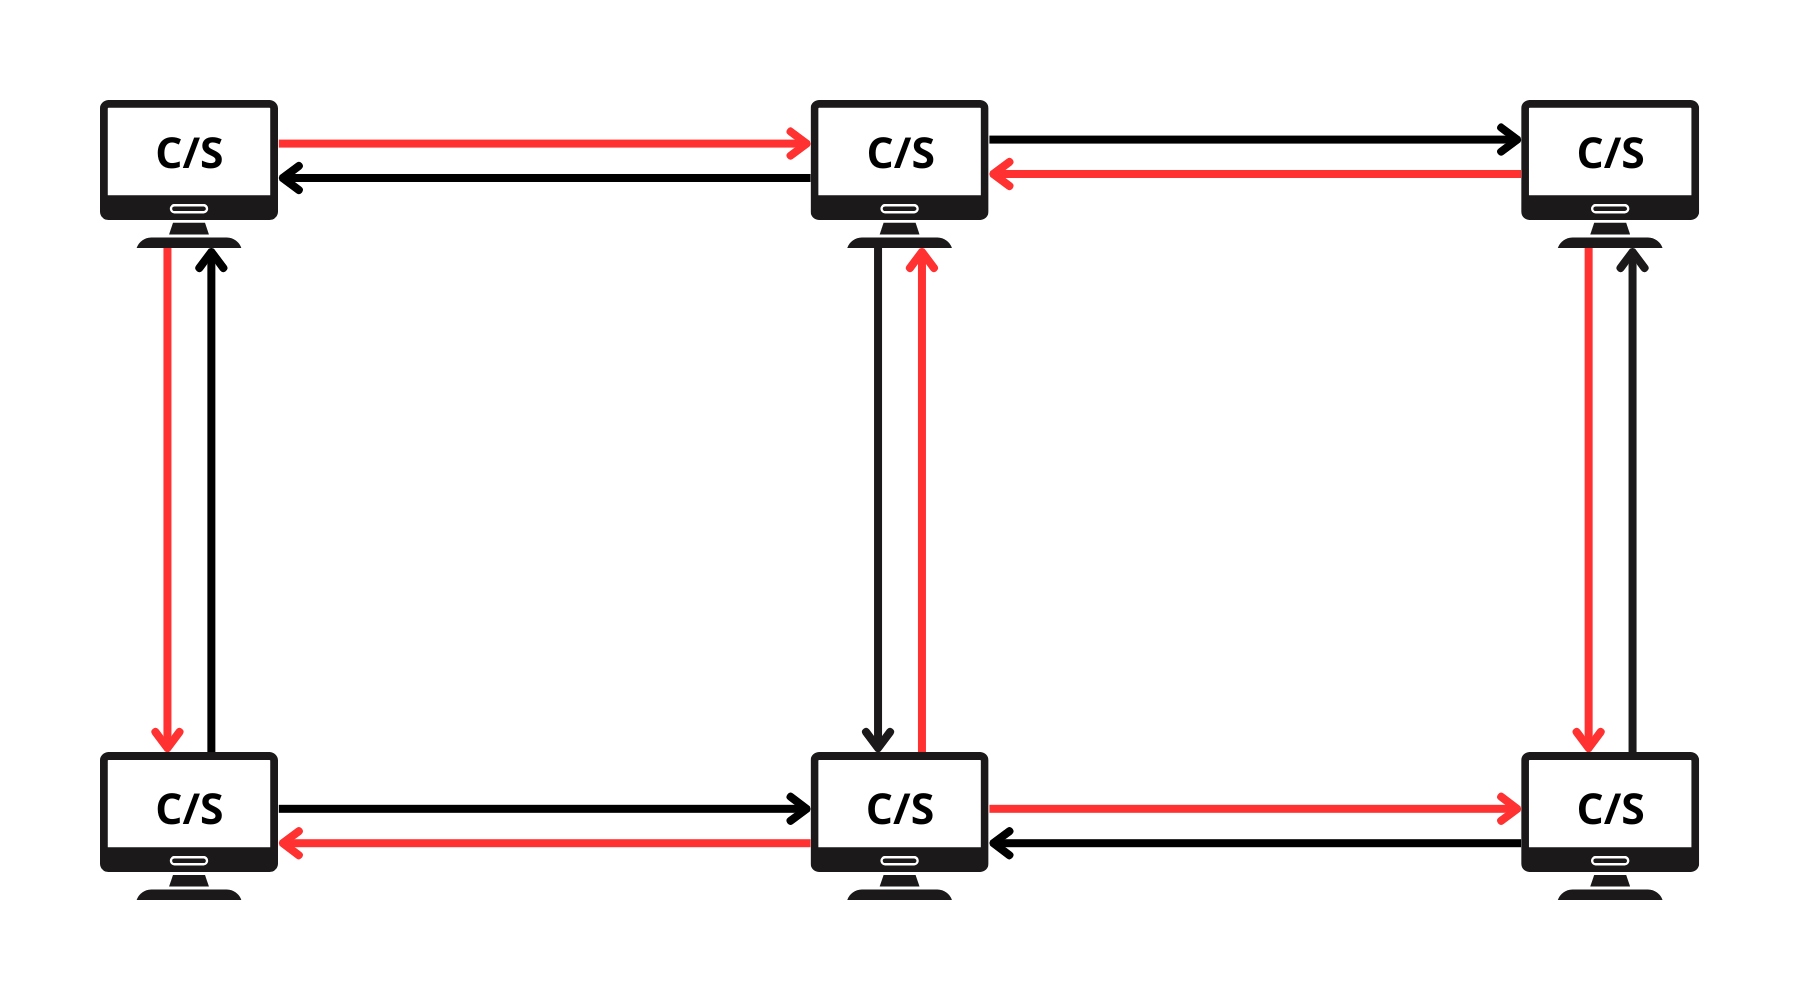
\includegraphics[width=\linewidth]{img/p2p.png}
            \caption{{creata con \href{https://www.canva.com/}{Canva}}}
        \end{figure}
        \tiny{
            \textbf{Curiosità}\\
            \href{https://ipfs.tech/}{InterPlanetary File System} (IPFS), 
            \href{https://www.insidemarketing.it/ipfs-come-funziona}{come funziona?}\\
        }
    \end{columns}
\end{frame}

\section{EVOLUZIONE E SERVIZI DI INTERNET}

\begin{frame}{EVOLUZIONE DI INTERNET}
    \begin{itemize}
        \justifying
        \item \textbf{WEB 1.0}: Contenuti statici. Anche nel caso in cui le pagine contenessero immagini o video, 
        il loro scopo rimaneva comunque la consultazione passiva da parte dell’utente. Non era prevista 
        interazione tra il visitatore e il contenuto;\\
        \begin{tiny}
            \raggedleft
            \textbf{Curiosità}\\
            \href{https://www.ilpost.it/massimomantellini/2021/10/11/internet-in-effetti-si-e-rotta/}{Internet, in effetti, si è rotta} e 
            \href{https://archive.org/}{Internet Archive}\\
        \end{tiny}
        \pause
        \item \textbf{WEB 2.0}: Tim O’Reilly nella sua \href{https://en.wikipedia.org/wiki/Web\_2.0\_Summit}{Web 2.0 Conference} del 2004 definì un nuovo Internet 
        dinamico, in cui le applicazioni diventavano in grado di interagire attivamente con l’utente. Si aggiunge 
        la possibilità di creare contenuti, di commentarli e di condividerli. Nascono i social network, i blog, 
        i forum, le piattaforme di video sharing e di file sharing;\\
        \begin{tiny}
            \raggedleft
            \textbf{Curiosità}\\
            \href{https://quantsmagazine.com/2024/10/e-ancora-possibile-salvare-internet/}{\'E ancora possibile salvare Internet?}\\
        \end{tiny}
        \pause
        \item Il futuro \textbf{WEB 3.0}: Propone a un rapporto ancora più approfondito tra uomo e macchina. 
        Si parla di \textbf{“read-write-interact web”}: un web in cui l’utente potrà ``leggere", ``scrivere", ma 
        anche ``interagire" in maniera più ampia e libera.\\
        \begin{tiny}
            \raggedleft
            \textbf{Curiosità}\\
            \href{https://it.wikipedia.org/wiki/Teoria_di_Internet_morto}{Dead Internet Theory}\\
        \end{tiny}
    \end{itemize}
\end{frame}

\begin{frame}{SERVIZI DI INTERNET}
    \begin{columns}
        \column{.8\textwidth}
        \begin{figure}
            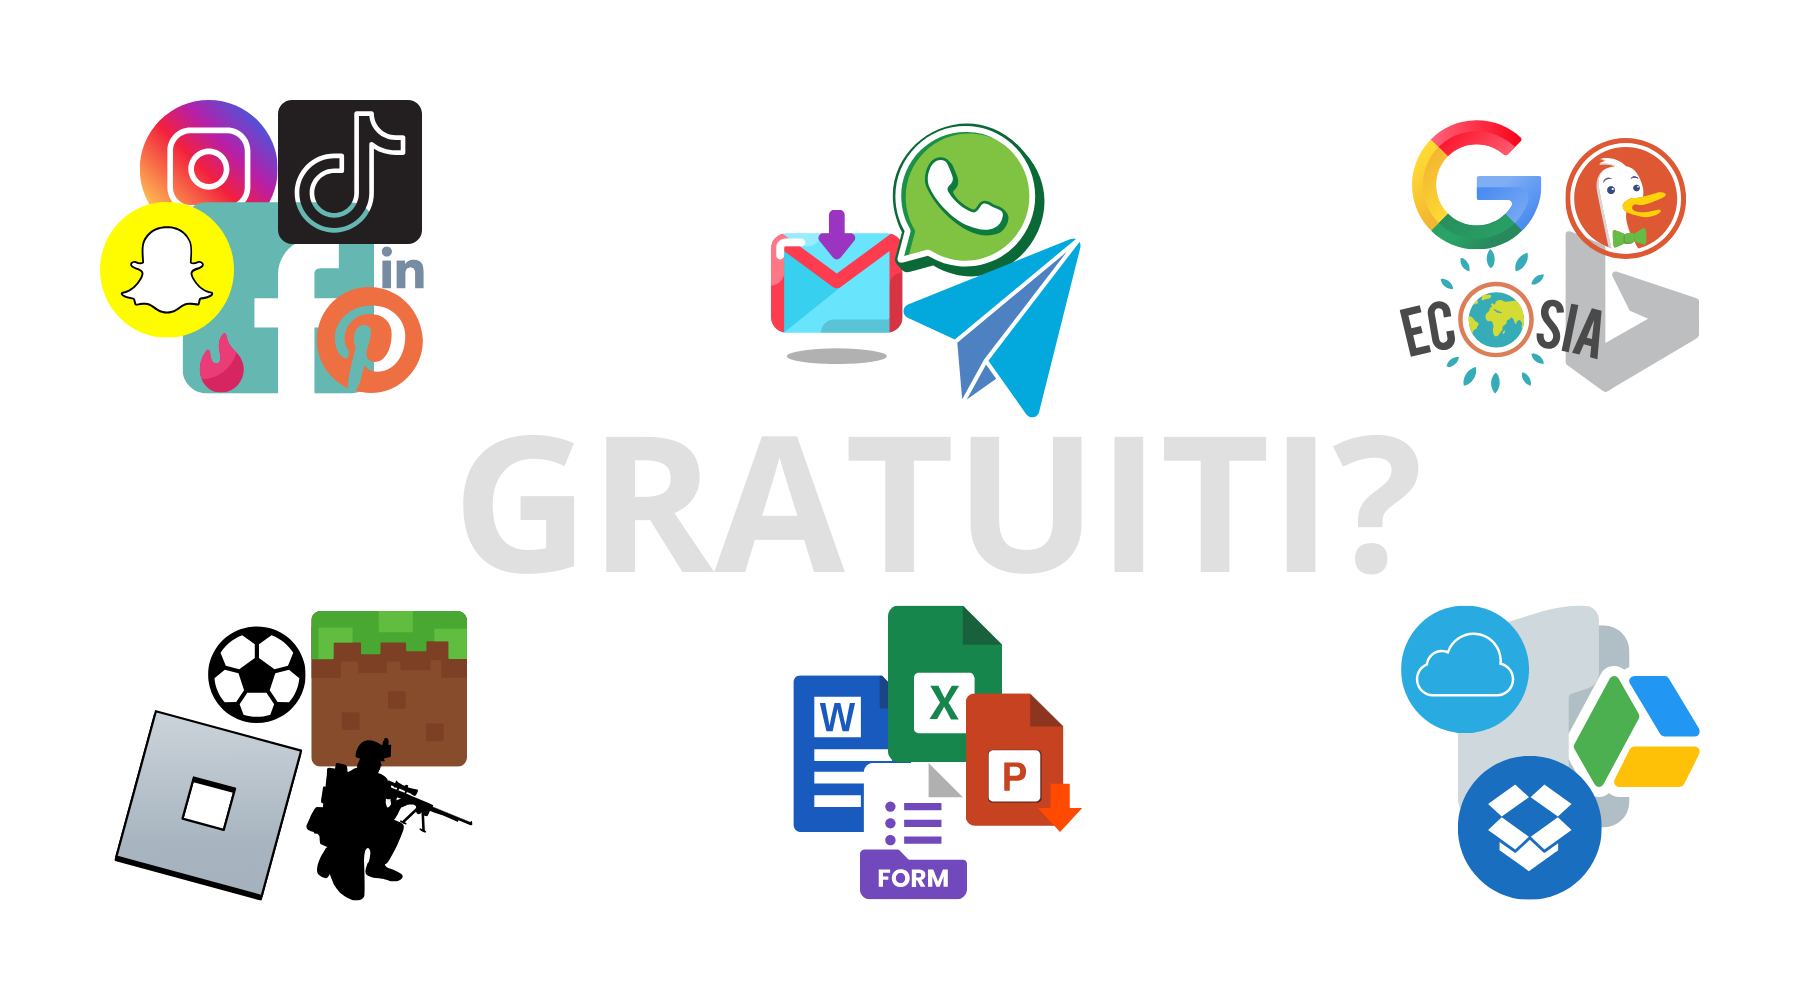
\includegraphics[width=\linewidth]{img/servizi_Internet.png}
            \caption{{creata con \href{https://www.canva.com/}{Canva}}}
        \end{figure}
        \tiny{
            \textbf{Curiosità}\\
            \href{https://mastodon.it/}{Mastodon} e 
            \href{https://www.rsi.ch/web/podcast/il-disinformatico/Mastodon-e-fediverso-perch\%C3\%A9-se-ne-parla-cos\%C3\%AC-tanto--1600469.html}{Fediverso} 
            (\href{https://it.wikipedia.org/wiki/ActivityPub}{ActivityPub})\\
            \href{https://www.linkiesta.it/blog/2015/11/la-storia-della-regola-34-di-internet/}{Regola 34 di Internet}\\
        }
    \end{columns}
\end{frame}

\end{document}